% Chapter 1 is an English rendering of บทที่ 1 บทนำ in the faculty template
% (docs/MyThesisInfo/final_report.pdf, pp. 1-3).  The objectives and scope are
% those the project was proposed with; which of them the implemented system
% addresses is recorded in Chapter 3 (section 3.1 and table 3.x, deviations),
% not rewritten here.
% The contents groups the chapters under a CHAPTER line; it is written from
% here rather than main.tex because \include emits its aux pointer immediately.
\addtocontents{toc}{\protect\vspace{6pt}\protect\noindent\protect\textbf{CHAPTER}\par}
\chapter[INTRODUCTION]{Introduction}
\label{chap:introduction}

\section{Background and Significance}
\label{sec:background}

Autonomous mobile robots (AMRs) play a central role in raising the efficiency of
warehouse logistics. Gensurv Robotics currently relies on 2-D LiDAR sensing
combined with QR-code navigation. That solution carries business limitations:
LiDAR sensors are expensive, and the approach is inflexible because the company
must spend money and time modifying the warehouse infrastructure to install
artificial reference markers. Moving from LiDAR to vision-based navigation,
which uses lower-cost camera sensors and yields richer information about the
environment, is therefore an option that directly addresses the company's cost
problem.

Bringing cameras and simultaneous localization and mapping from images (visual
SLAM) into real warehouse use nevertheless raises a substantial academic
challenge. Most standard visual SLAM algorithms were developed under the
assumption that the environment is static. Saputra et al.~\cite{saputra2018}
state clearly that when a SLAM system is deployed in a dynamic environment, such
as a warehouse in which goods and obstacles are continually moved, its accuracy
degrades severely, because the system draws features from moving objects into
its pose computation. Cadena et al.~\cite{cadena2016} further stress that the
greatest challenges facing SLAM today are robustness and lifelong mapping: the
robot must be able to separate permanent structure from dynamic objects.

To address navigation in a dynamic environment, this project proposes the
development of a vision-based navigation pipeline centred on integrating the
YOLO26 deep-learning model to detect and filter dynamic objects out of the
localization system. The project develops and compares the performance of two
navigation-system architectures: (1) operation with the ORB-SLAM3 framework, and
(2) operation with VINS combined with RTAB-Map, in order to find the most robust
approach for a warehouse.

In addition, replacing an active sensor (LiDAR) with a passive one (a camera)
may make the system sensitive to indoor lighting conditions. The project
therefore designs an experiment that simulates the environment and the light
intensity at different times of day, so that data can be collected and it can be
assessed empirically whether warehouse lighting significantly affects the
performance of the visual SLAM system. That assessment will be important input
to the company's long-term development and improvement of its navigation system.

\section{Objectives}
\label{sec:objectives}

\begin{enumerate}[leftmargin=2em]
  \item Develop a visual-inertial odometry localization system with lifelong
    mapping, so that the warehouse map is updated in real time.
  \item Develop image enhancement for low-light environments with the
    EnlightenGAN model.
  \item Develop perception of obstacles and moving objects (dynamic objects)
    through deep-learning object detection.
  \item Develop lane detection with PolyNET and lane tracking with a PID
    controller.
  \item The integrated system must be able to build a 2-D cost map and localize
    the robot with an error of less than \SI{10}{\centi\metre} under differing
    light intensities.
\end{enumerate}

\section{Expected Benefits}
\label{sec:benefits}

\begin{enumerate}[leftmargin=2em]
  \item Help the company reduce the cost of modifying warehouse infrastructure
    for AMR navigation.
  \item Obtain a navigation pipeline that is robust to a dynamic environment.
  \item Allow the pipeline to be plugged into the control and motion-planning
    systems for real use on warehouse robots.
\end{enumerate}

\section{Scope}
\label{sec:scope}

\begin{enumerate}[leftmargin=2em]
  \item The main tests are carried out only on a small mobile robot computing on
    an NRU-51V processing unit and using AC-IMX390-H190 cameras.
  \item Within the AMR navigation system, the author's work is framed only
    within the visual SLAM, object prediction and lane-tracking controller
    blocks (red frame) shown in \cref{fig:scope-architecture}.
  \item The integrated system is tested only in a mock warehouse arena with
    changing mock goods, a walkway with a \SI{5}{\degree} slope, five stacks of
    goods of four boxes each, and a starting point at the grey square at the
    lower right of \cref{fig:test-field}. The positions of the mock warehouse
    contents are changed between tests to simulate a dynamic environment.
\end{enumerate}

\begin{figure}[htbp]
  \centering
  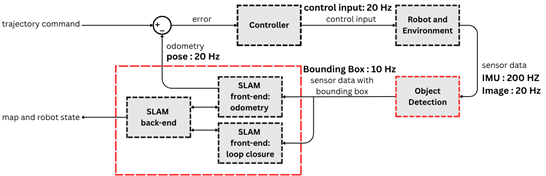
\includegraphics[width=0.9\textwidth]{figures/template/control_loop_rates.png}
  \caption[Scope of the project within the AMR navigation loop.]{Scope of the project within the AMR navigation loop. The red dashed
  frame encloses the blocks this project develops: the SLAM front end
  (odometry and loop closure), the SLAM back end (map and robot state) and the
  object-detection block that supplies bounding boxes. The controller and the
  robot are existing components. Rates are those of the target system: control
  input \SI{20}{\hertz}, odometry pose \SI{20}{\hertz}, bounding boxes
  \SI{10}{\hertz}, IMU \SI{200}{\hertz}, images \SI{20}{\hertz}.}
  \label{fig:scope-architecture}
\end{figure}

\begin{figure}[htbp]
  \centering
  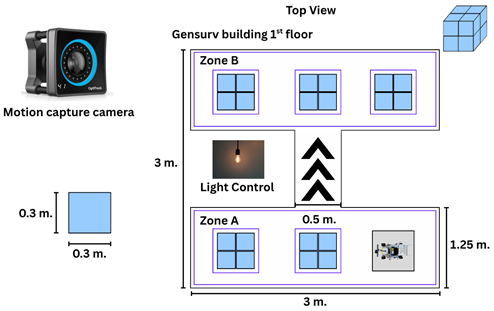
\includegraphics[width=0.8\textwidth]{figures/template/test_field_topview.png}
  \caption[Top view of the mock warehouse test field on the first floor of the Gensurv building.]{Top view of the mock warehouse test field on the first floor of the
  Gensurv building. Zone~A and Zone~B are each \SI{3}{\metre} square and are
  joined by a walkway; the robot starts at the grey square in Zone~A. Goods are
  \SI{0.3}{\metre} cubes stacked in piles, a light-control fixture sets the
  illumination, and motion-capture cameras around the field provide the
  ground-truth reference.}
  \label{fig:test-field}
\end{figure}

\section{Work Plan}
\label{sec:workplan}

\Cref{tab:gantt} reproduces the project work plan of the proposal. Task
numbering follows the original plan, which has no item~5.

\begin{table}[htbp]
\centering
\caption[Work plan for the 2026 (B.E.\ 2569) academic year.]{Work plan for the 2026 (B.E.\ 2569) academic year. Shaded cells mark
the months allocated to each task.}
\label{tab:gantt}
\small
\setlength{\tabcolsep}{3pt}
\newcommand{\gc}{\cellcolor{black!12}}
\begin{tabularx}{\textwidth}{>{\raggedright\arraybackslash}X ccccccc}
\toprule
Task & Jun & Jul & Aug & Sep & Oct & Nov & Dec \\
\midrule
1. Study the concepts and theory of vision-based navigation
  & \gc & \gc & & & & & \\
2. Search and analyse information on visual SLAM algorithms, low-light image
  enhancement (EnlightenGAN), object detection (YOLO26) and lane tracking
  (PolyNET)
  & \gc & \gc & & & & & \\
3. Design the structure and software pipeline that joins the hardware and
  software systems
  & & \gc & \gc & & & & \\
4. Specify and connect the AC-IMX390-H190 camera sensors with the NRU-51V edge
  computing unit on the mobile robot
  & & \gc & \gc & & & & \\
6. Integrate all subsystems under the AMR navigation framework
  & & & \gc & \gc & & & \\
7. Prepare the mock warehouse area (Zone~A and Zone~B) with a \SI{5}{\degree}
  slope and arrange mock goods to create a dynamic environment
  & & & \gc & \gc & & & \\
8. Run the integrated system experiment (live test) with the robot moving at
  \SI{1.5}{\metre\per\second} under scheduled changes in lighting
  & & & & \gc & \gc & & \\
9. Collect the test data and evaluate system performance on the defined
  metrics: trajectory error (ATE, RPE), system latency, and detection accuracy
  (IoU, mAP)
  & & & & & \gc & \gc & \\
10. Summarise the work, discuss the results and produce the complete
  engineering project report
  & & & & & & \gc & \gc \\
\bottomrule
\end{tabularx}
\end{table}
